\chapter{Implementación y Diseño}
	\section{Introducción}
	Debido a que se adoptó un modelo de desarrollo en espiral se plantearon una serie de prototipos que incluyen mayor funcionalidad en cada iteración
	del modelo. Inicialmente se planteó un prototipo de básico para determinar factibilidad de puesta en funcionamiento de un SoC con microprocesador
	OpenRISC y el desarrollo de aplicaciones que se ejecuten en él. Debido a su funcionalidad reducida y menor consumo de recursos  para su síntesis se
	seleccionó el proyecto MinSoC para el desarrollo del primer prototipo con el cual se evaluaron y documentaron las capacidades del mismo permitiendo
	valorar este proyecto para aplicaciones donde no se requieren grandes cantidades de memoria y juegan un papel primordial las entradas/salidas junto
	a la capacidad de procesamiento.  
		 
		\subsection{Entorno de ejecución}
		Actualmente OpenRISC es soportado por un conjunto de herramientas de desarrollo(toolchain) de 32 bits ofreciendo soporte para los lenguajes C y C++
		con librerías estáticas. El toolchain se encuentra disponible en dos formas: una para la ejecución de aplicaciones bajo el sistema operativo Linux y
		otra para la ejecución de aplicaciones standalone o bare metal que son aquellas que se ejecutan e interactúan directamente con el hardware sin la
		necesidad de un sistema operativo que proporcione soporte para la utilización de los periféricos.
		
			\subsubsection{Entorno de ejecución Standalone - Bare Metal}
	    	Para la ejecución de aplicaciones Bare Metal el toolchain se basa en la librería newlib que es una implementación estándar utilizada en
	    	sistemas embebidos. 
	    
			\subsubsection{Entorno de ejecución Linux}
			Por otro lado, para el uso de aplicaciones bajo el sistema operativo Linux el toolchain puede ser compilado en base a la librería uClibc que es la
			opción para sistemas embebidos de la librería glibc utilizada en los sistemas estándar.
		
		\subsection{Criterio para la realización de testing}%%corregir esto
		El testing desarrollado apunta verificar el cumplimiento de los requerimientos individualmente e incrementalmente. Se pretende utilizar las
		aplicaciones de prueba provistas y desarrollar algunas que verfiquen los requerimientos de compilación , depuración y ejecución de aplicaciones para
		openRISC. 
Los testing sirven para poder detectar la presencia de errores, pero aún si un testing no arroja resultados erróneos, esto no nos garantiza el correcto funcionamiento del sistema 
El tipo de testing realizado es de verificación. La verificación es el proceso de evaluación de un sistema o componente para determinar si el producto cumple con lo que se ha diseñado, es decir, si cada fase de desarrollo dado cumplen con los requisitos impuestos al inicio de dicha fase

\newpage
	\section{PROTOTIPO UNO: Implementación del SoC MinSoC en FPGA}
		\subsection{Introducción}
		
	En este primer prototipo se implementó el proyecto MinSoC en la placa de desarrollo S3ADSP1800A con el fin de verificar el funcionamiento del procesador y sus periféricos. Para lograr este objetivo se requiere de la instalación y puesta en funcionamiento de las herramientas de síntensis, place \& route(PAR) y programación de la FPGA Spartan 3A. 

		\subsection{Requerimientos del prototipo}
		\begin{table}[h]
		\centering
		\begin{tabular}{ p{2.5cm} p{8cm} p{3cm} }
		\hline 
		\rowcolor[gray]{0.8} N\textordmasculine Req & Descripción\\
		\hline 
		RQX-PA 1 & El prototipo debe implementar un SoC MinSoC en la placa desarrollo S3ADSP1800A\\ 
		\hline 
		RQX-PA 2 & El prototipo debe garantizar el correcto funcionamiento de todos los periféricos conectados al SoC mediante el bus Wishbone\\ 
		\hline 
		RQX-PA 3 & El prototipo debe interactuar correctamente con las interfaces hardware soportadas de la placa de desarrollo S3ADSP1800A\\ 
		\hline
		RQX-PA 4 & El prototipo debe ser capaz de ejecutar programas con capacidad de depuración generados mediante compilación
		cruzada en una arquitectura x86 y/o x86\_64 para arquitectura la OpenRISC\\
		\hline
		RQX-PA 5 & Se debe lograr depurar paso a paso y mediante break points las aplicaciones desarrolladas\\
		\hline		
		\end{tabular}
		\end{table}
		
\newpage
		\subsection{Descripción de la Arquitectura}
	
		La Figura ~\ref{fig:minsoc} muestra un esquema de la arquitectura planteada en el prototipo. Se utiliza un estación de trabajo corriendo las
		herramientas de compilación (GCC) y depuración (GDB) en sus versiones de compilación cruzada para arquitecturas destino openRISC. Se requiere de un
		servidor que proporcione un puerto para la depuración con GDB , acción realizada por la aplicación Advanced JTAG Bridge que provee la interfase de
		comunicación entre el TAP JTAG conectado al SoC a través el cable JTAG y la estación de trabajo.
		
		\begin{figure}[!h]
 		\begin{center}
  		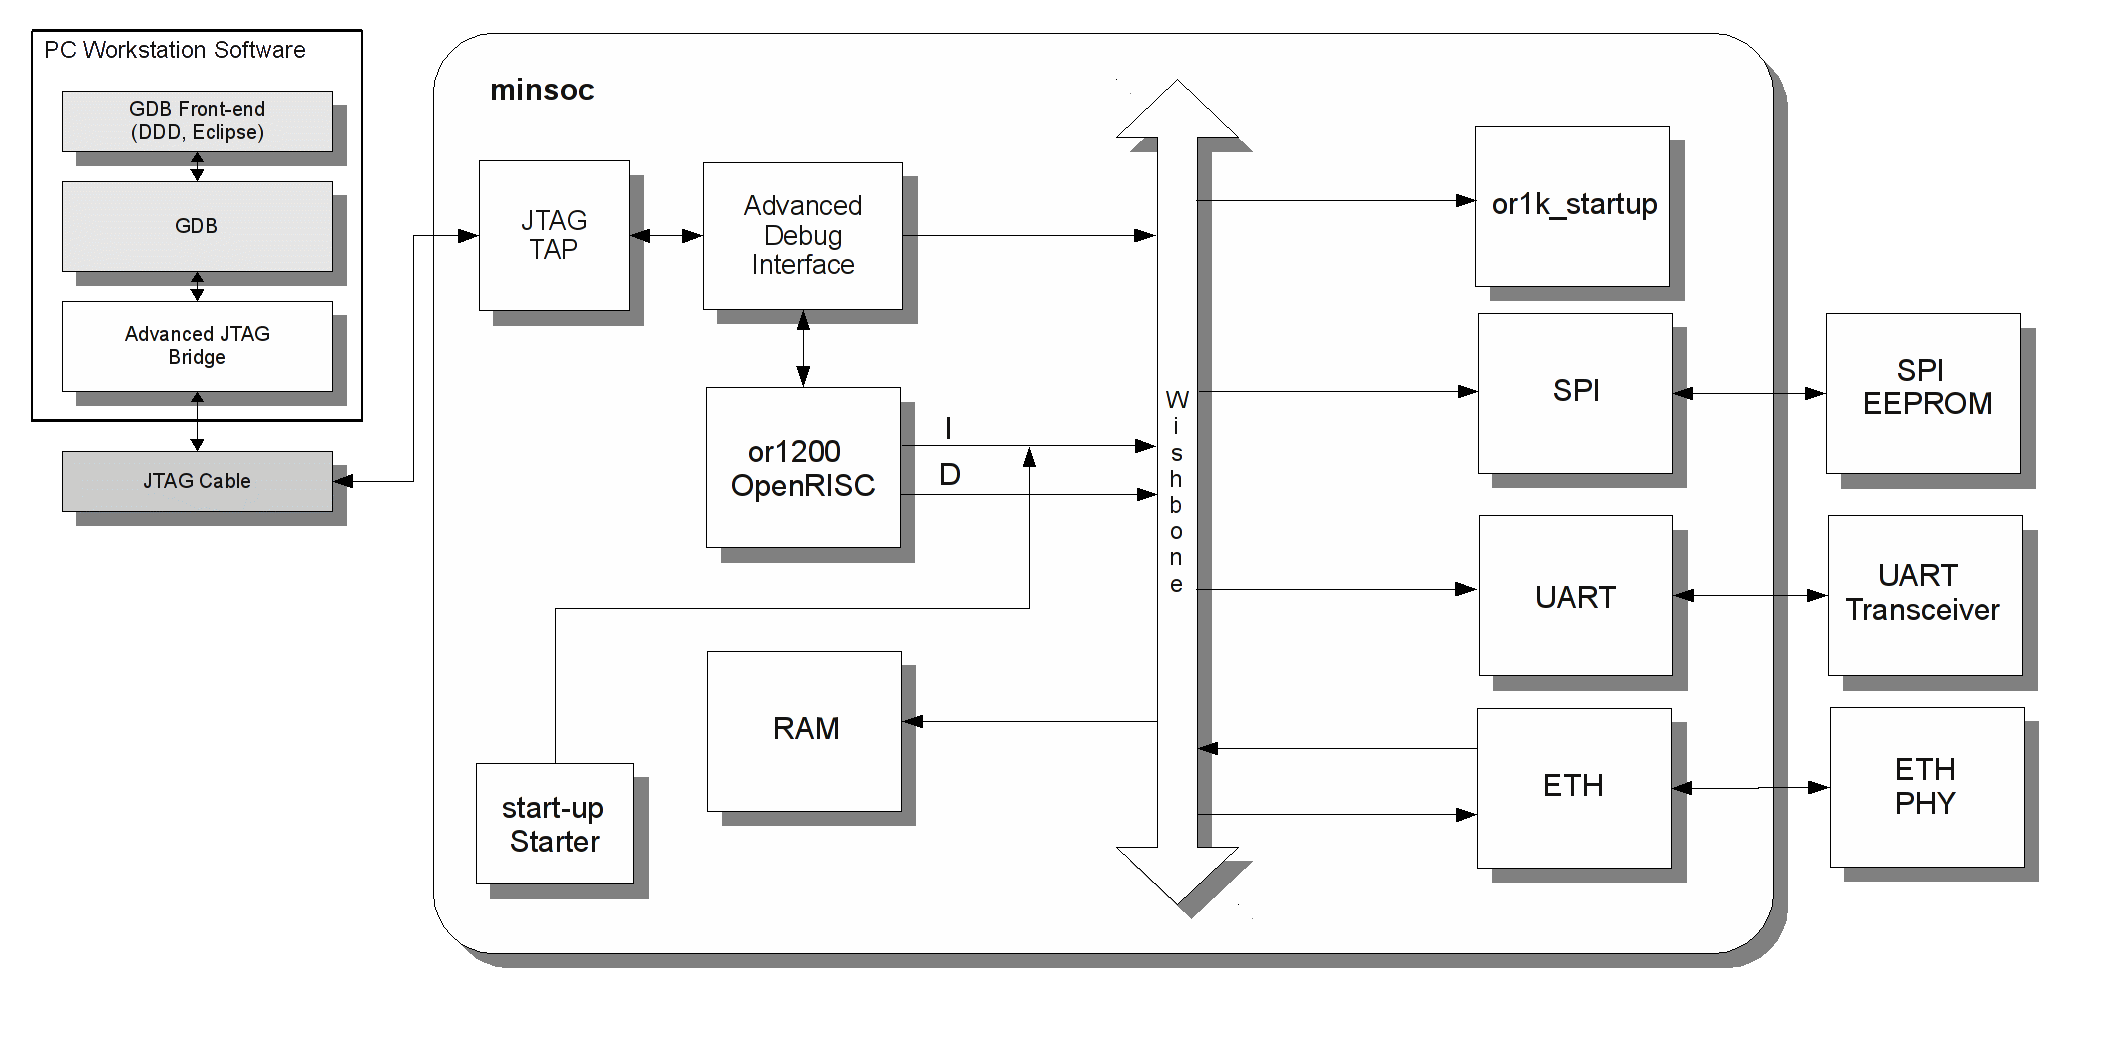
\includegraphics[width=1\textwidth,keepaspectratio=true]{./images/minsoc}
  		\caption{Arquitectura Prototipo 1}
  		\label{fig:minsoc}
 		\end{center}
		\end{figure}
		
		El módulo Advanced Debug Interface proporciona soporte para la depuración via JTAG, está conectado directamente al microprocesador y a su vez al bus
		general Wishbone donde se conectan el resto de los periféricos. Se conectan al sistema mediante el bus antes mencionado : un modulo	de RAM
		sintetizado, un módulo de arranque (startup), un módulo SPI que interactúa con la memoria flash on board de la placa S3ADSP1800A , un módulo UART y
		un módulo ETHERNET. El sistema inyecta un pequeño código de arranque directamente al bus de instrucciones al iniciar o luego de un reset. 
			
		\subsection{Implementación}
		\subsubsection{Síntesis , PAR , Generación del bitfile del proyecto}
%%%%%%%%%%%%%%%%%%%%%into al tema%%%%%%%%%%%%%%%		
La implementación se realiza normalmente en cinco pasos básicos: 
\begin {itemize}
\item Descarga del script de instalación.
\item Ejecución del script de instalación.
\item Configuración de la placa especifica para la síntesis.
\item Generación del flujo de bits.
\item Programación de la FPGA Spartan 3a.
 \end {itemize}
 Consulte la Guía de MinSoc en el Anexo1 para una comprensión más profunda de los pasos a seguir en la implementación sobre la placa de desarrollo S3ADSP1800A.

		
		\subsubsection{Configuración de la FPGA}
		Este proceso de grabación se realizó mediante las herramientas del fabricante (iMPACT) y mediante un herramienta Open Source llamada xc3sprog. 
		
		%%%%%%%\subsection{Diagrama de Secuencia}
		%%%%%%%%%%agregar al anexo xc3cprog
%%%%%%%%%%%%%%%%%%%%%%%%%%%%%%%%%%%%%testing%%%%%%%%%%%%%%%%%%		
		\subsection{Testing de Requerimientos del Prototipo1}

%%%%%%%%%%%%%%%%%%%%%%%REQ 1%%%%%%%%%%%%%%%%%%
		
%%%%%%%%%%%%%%%%%%%%%%%REQ 2%%%%%%%%%%%%%%%%%%

%%%%%%%%%%%%%%%%%%%%%%%REQ 3%%%%%%%%%%%%%%%%%%
\begin{table}[!h]
		\centering
		\begin{tabular}{ p{5cm} p{10cm}  }
		\hline 
	\rowcolor[gray]{0.8}  Caso de Prueba&  Interactuar correctamente con las interfaz hardware UART\\
		\hline 
		Código de Requerimiento & RQX-PA 3\\ 
		\hline 
		Requerimiento  &  El prototipo debe interactuar correctamente con las interfaces hardware soportadas de la placa de desarrollo S3ADSP1800A\\ 
		\hline 
		Código de Testing & T003\\ 
		\hline
		Propósito &  \\
		\hline
		Realizado Por & Gomez, Pablo \\
		\hline	
		Entorno de Ejecución & Bare Metal \\
		\hline
		Precondiciones &  \\
		\hline
		Secuencia de Ejecución &  \\
		\hline
		Postcondiciones & \\
		\hline
		\rowcolor[gray]{0.8}  v&Resultados\\
		\hline
		Resultados Esperados & Poder observar por la terminal serial una cadena de string.\\
		\hline	
		Resultados Obtenidos & Al ejecutarse la aplicación de prueba del uart se pudo observar la cadena de string esperada "HELLO WORLD" \\
		\hline
		\end{tabular}
		\end{table}

\begin{table}[!h]
		\centering
		\begin{tabular}{ p{5cm} p{10cm}  }
		\hline 
	\rowcolor[gray]{0.8}  Caso de Prueba&  Interactuar correctamente con las interfaces hardware de Ethernet\\
		\hline 
		Código de Requerimiento & RQX-PA 3\\ 
		\hline 
		Requerimiento  &  El prototipo debe interactuar correctamente con las interfaces hardware soportadas de la placa de desarrollo S3ADSP1800A\\ 
		\hline 
		Código de Testing & T004\\ 
		\hline
		Propósito &  El envío de paquetes de Ethernet mediante broadcast desde el SoC  \\
		\hline
		Realizado Por & Gomez, Pablo \\
		\hline	
		Entorno de Ejecución & Bare Metal \\
		\hline
		Precondiciones &  \\
		\hline
		Secuencia de Ejecución &  \\
		\hline
		Postcondiciones & \\
		\hline
		\rowcolor[gray]{0.8}  v&Resultados\\
		\hline
		Resultados Esperados & Poder observar por la terminal serial una cadena de string indicando el inicio del envío de paquetes Ethernet y verificar la llegada de los mismos por medio de una aplicación sniffer \\
		\hline	
		Resultados Obtenidos & Al ejecutarse un programa de prueba pudo observarse la cadena de strig "HELLO WORLD" y observar la cadena 0xFF02B4050" \\
		\hline
		\end{tabular}
		\end{table}


\newpage
%%%%%%%%%%%%%%%%%%%%%%%REQ 4%%%%%%%%%%%%%%%%%%
\begin{table}[!h]
		\centering
		\begin{tabular}{ p{5cm} p{10cm}  }
		\hline 
		\rowcolor[gray]{0.8}  Caso de Prueba& Ejecución de la aplicación multiplicadora de matrices binarias  desarrollada \\
		\hline 
		Código de Requerimiento & RQX-PA 4\\ 
		\hline 
		Requerimiento  &  El prototipo debe ser capaz de ejecutar programas con capacidad de depuración, generados mediante compilación cruzada en una arquitectura x86 y/o x86\_64 para arquitectura la OpenRISC\\ 
		\hline 
		Código de Testing & T005\\ 
		\hline
		Propósito &  Compilación y Ejecución de un  programa sencillo en c.Verificar si el sistema de hardware está funcionando y  prueba del entorno de desarrollo de software. \\
		\hline
		Realizado Por & Gomez, Pablo \\
		\hline	
		Entorno de Ejecución & Bare Metal \\
		\hline
		Precondiciones & descarga e instalación del complicador cruzado \\
		\hline
		Secuencia de Ejecución &  \\
		\hline
		Postcondiciones & \\
		\hline
		\rowcolor[gray]{0.8}  v&Resultados\\
		\hline
		Resultados Esperados & \\
		\hline	
		Resultados Obtenidos & \\
		\hline
		\end{tabular}
		\end{table}
\newpage
%%%%%%%%%%%%%%%%%%%%%%%REQ 5%%%%%%%%%%%%%%%%%%

\begin{table}[!h]
		\centering
		\begin{tabular}{ p{5cm} p{10cm}  }
		\hline 
		\rowcolor[gray]{0.8}  Caso de Prueba&  Se debe lograr depurar paso a paso y mediante break points las aplicaciones desarrolladas\\
		\hline 
		Código de Requerimiento & RQX-PA 5\\ 
		\hline 
		Requerimiento  &  Se debe lograr depurar paso a paso y mediante break points las aplicaciones desarrolladas\\ 
		\hline 
		Código de Testing & T002\\ 
		\hline
		Propósito &  \\
		\hline
		Realizado Por & Gomez, Pablo \\
		\hline	
		Entorno de Ejecución & Bare Metal \\
		\hline
		Precondiciones & Pasado con éxito los casos de prueba anteriores \\
		\hline
		Secuencia de Ejecución &  \\
		\hline
		Postcondiciones & \\
		\hline
		\rowcolor[gray]{0.8}  v&Resultados\\
		\hline
		Resultados Esperados & \\
		\hline	
		Resultados Obtenidos & \\
		\hline
		\end{tabular}
		\end{table}

\newpage


		\subsubsection{Modo de prueba de requerimientos}
		La capacidad de procesamiento del sistema se probó mediante alguno programas de cálculo matricial (matrices binarias).  
		
		Se utilizaron diferentes aplicaciones de prueba de periféricos para validar el correcto funcionamiento de los mismos. 
		
		\subsubsection{Diseño y selección de aplicaciones de prueba}
		\paragraph{Prueba del perisférico UART}
		Para la realización de este test se utilizó el programa 
		
		\paragraph{Prueba de procesamiento: Multiplicador de matrices binarias}
		Como primer programa de prueba se realizó un multiplicador de matrices binarias generadas mediante una Secuencia binaria pseudo aleatoria (PRBS). Se
		realizaron los productos con matrices cuadradas incrementando su tamaño iteración a iteración. 
		
		
		
		\subsubsection{Resultados obtenidos}
		
	
		\subsection{Conclusión}
		Se pudo implementar con éxito el prototipo número uno cuyos resultados muestran
\newpage
		
	\section{PROTOTIPO DOS: Implementación del SoC ORPSoc en FPGA}
		\subsection{Introducción}
		Para el prototipo dos se planteó la implementación de un SoC ORPSoC que dispone de mayor cantidad de periféricos que el MinSoC entre ellos un módulo
		que permite manejar las memorias RAM DDR2 incluídas en la placa de desarrollo S3ADSP1800A. Se verificó inicialmente si la herramientas utilizadas en
		el prototipo uno proporcionaban los mismos resultados en este prototipo y luego se ejecutaron las pruebas de funcionamiento del procesador, los
		periféricos y las herramientas de desarrollo y depuración. 
		
		\subsection{Requerimientos del prototipo}
		\begin{table}[h]
		\centering
		\begin{tabular}{ p{2.5cm} p{8cm} p{3cm} }
		\hline 
		\rowcolor[gray]{0.8} N\textordmasculine Req & Descripción\\
		\hline 
		RQX-PB 1 & El prototipo debe implementar un SoC ORPSoC en la placa desarrollo S3ADSP1800A\\ 
		\hline 
		RQX-PB 2 & El prototipo debe garantizar el correcto funcionamiento de todos los periféricos conectados al SoC mediante el bus Wishbone\\ 
		\hline 
		RQX-PB 3 & El prototipo debe interactuar correctamente con las interfaces hardware soportadas de la placa de desarrollo S3ADSP1800A\\ 
		\hline
		RQX-PB 4 & Se debe garantizar el acceso a las memorias RAM DDR2 de la plataforma S3ADSP1800A\\
		\hline
		RQX-PB 5 & El prototipo debe se capaz de ejecutar programas con capacidad de depuración generados mediante compilación
		cruzada en una arquitectura x86 y/o x86\_64 para arquitectura la OpenRISC\\
		\hline
		RQX-PB 6 & Se debe lograr depurar paso a paso y mediante break points las aplicaciones desarrolladas\\
		\hline
		RQX-PB 7 & El prototipo debe ser evaluado mediante el benchmark CoreMark para el posterior análisis de las capacidades del SoC\\
		\hline		
		\end{tabular}
		\end{table}

		\subsection{Descripción de la Arquitectura}

	
		\subsection{Implementación}

		
		\subsection{Diseño y selección de aplicaciones de prueba}
		
		
		\subsection{Testing}


		\subsection{Conclusión}


	\section{PROTOTIPO TRES: Implementación del SoC ORPSoC en FPGA con Sistema Operativo eCos}
		\subsection{Introducción}
		Para tercer prototipo se añadió al prototipo dos la funcionalidad aportada por el Sistema Operativo eCos(embedded configurable operating system) que
		adiciona la capacidad de ejecución un proceso con múltiples hilos. 

		\subsection{Requerimientos del prototipo}

		\begin{table}[h]
		\centering		
		\begin{tabular}{ p{2.5cm} p{8cm} p{3cm} }
		\hline 
		\rowcolor[gray]{0.8} N\textordmasculine Req & Descripción\\
		\hline 
		RQX-PC 1 & El prototipo debe implementar el sistema operativos eCos\\ 
		\hline 
		RQX-PC 2 & Se deben garantizar el correcto funcionamiento de todos los periféricos utilizando las librerias provistas por el SO\\ 
		\hline 
		RQX-PC 3 & Se requiere la ejecución de múltiples hilos y la ejecución de programas de prueba para determinar los límites de esta capacidad \\ 
		\hline
		RQX-PC 4 & \\
		\hline
		RQX-PC 5 & \\
		\hline
		RQX-PC 6 & \\
		\hline
		RQX-PC 7 & \\
		\hline		
		\end{tabular}
		\end{table}
		
		
		\subsection{Implementación}
		
		\subsection{Testing}
		
		\subsection{Conclusión}
		
		
	\section{PROTOTIPO CUATRO: Implementación del SoC ORPSoC en FPGA con Sistema Operativos Linux}
		\subsection{Introducción}
		El núcleo Linux, combinado con un conjunto de algunas otras utilidades de software libre, puede ajustarse dentro del limitado espacio de hardware 
	    de los sistemas embedidos. Una instalación típica de un Linux embebido ocupa en promedio 2 MB. En el prototipo cuatro se utilizó una versión
	    reducida del núcleo de Linux y herramientas provistas por el paquete BusyBox. 
		
		\subsection{Requerimientos del prototipo}
		
		\begin{table}[h]
		\centering	
		\begin{tabular}{ p{2.5cm} p{8cm} p{3cm} }
		\hline 
		\rowcolor[gray]{0.8} N\textordmasculine Req & Descripción\\
		\hline 
		RQX-PC 1 & El prototipo debe implementar el sistema operativos eCos\\ 
		\hline 
		RQX-PC 2 & Se deben garantizar el correcto funcionamiento de todos los periféricos utilizando las librerias provistas por el SO\\ 
		\hline 
		RQX-PC 3 & Se requiere la ejecución de múltiples hilos y la ejecución de programas de prueba para determinar los límites de esta capacidad \\ 
		\hline
		RQX-PC 4 & \\
		\hline
		RQX-PC 5 & \\
		\hline
		RQX-PC 6 & \\
		\hline
		RQX-PC 7 & \\
		\hline		
		\end{tabular}
		\end{table}
		
		
		\subsection{Implementación}
		
		\subsection{Testing}
		
		\subsection{Conclusión}
